\documentclass{AeroStructure-ERJohnson}
\input crosslink.tex

%\usepackage{showframe}
\def\ShowFrameLinethickness{0.125pt}

\myexternaldocument{App_4P}
%\myexternaldocument{Ch01_4P}
\myexternaldocument{Ch02_4P}
\myexternaldocument{Ch03_4P}
\myexternaldocument{Ch04_4P}
\myexternaldocument{Ch05_4P}
\myexternaldocument{Ch06_4P}
\myexternaldocument{Ch07_4P}
\myexternaldocument{Ch08_4P}
\myexternaldocument{Ch09_4P}
\myexternaldocument{Ch10_4P}
\myexternaldocument{Ch11_4P}
\myexternaldocument{Ch12_4P}
\myexternaldocument{Ch13_4P}
\myexternaldocument{Ch14_4P}
\myexternaldocument{Ch15_4P}
\myexternaldocument{Ch16_4P}
\myexternaldocument{Ch17_4P}
\myexternaldocument{Ch18_4P}


\begin{document}

\mainmatter

\chapter{Function of flight vehicle structural members}\label{ch1}

The purpose of this chapter is to present a brief description of aircraft
structural members and their function.


A structure may be defined as any assemblage of materials that is intended
to sustain loads. It is important to recognize that structures are made from
materials, and that the history of structures follows the development of
materials and the development of tools to fabricate the materials. Ashby
(1992) details a systematic approach to material selection in mechanical
design, and the manufacturing processes required produce the functional
shape of a design. The evolution of the airframe, for example, is tied
closely to the introduction of materials and cost-effective means for their
fabrication. Early aircraft were constructed of wire-braced wood frames with
fabric covers. Currently, advanced composite materials are very attractive
for weight-sensitive structures, like aircraft, because of their high
stiffness-to-weight and strength-to-weight ratios. There is an interesting
and rich history of the evolution of aircraft structures, but for the sake
of brevity it is not presented here. Instead, the interested reader is
referred to the textbook by Curtis (1997). Curtis details the history of
fixed--wing aircraft structures from 1903 to modern aircraft.


In this text analytical methods are developed for the response and failure
of the primary structural components of aircraft. The primary structure of a
flight vehicle consists of the components that are necessary to sustain
design ultimate flight and ground loads. Failure of the primary structure
causes catastrophic collapse and loss of control. For aircraft the primary
structure consists of the wings, fuselage, tail, and landing gear. Forms of
construction are space trusses/frames, monocoque and semimonocoque.


\section{Space truss/frame}

A truss structure fuselage is often used in lightweight aircraft.
See figure \ref{fig1.1}. It consists of wood or steel tubes with a fabric
covering providing aerodynamic shape. Members in a space truss are
subject to axial forces, and members of a space frame are subject
to axial forces, shear forces, and bending moments. The fabric
covering does not add much to the overall stiffness of the
structure.

\newpage

{\def\thefigure{1.1}
\begin{figure}
\centering{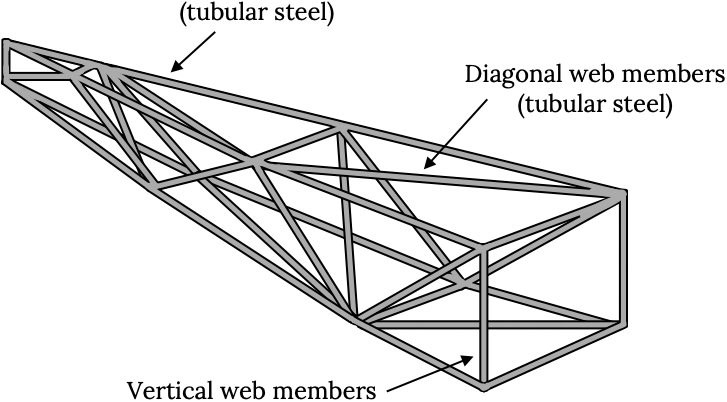
\includegraphics{Figure_1-1.pdf}}
\caption{A fuselage space frame structure.\label{fig1.1}}\vspace*{-20pt}
\end{figure}
}
{\def\thefigure{1.2}
\processfigure[b]{\vspace*{-6pt}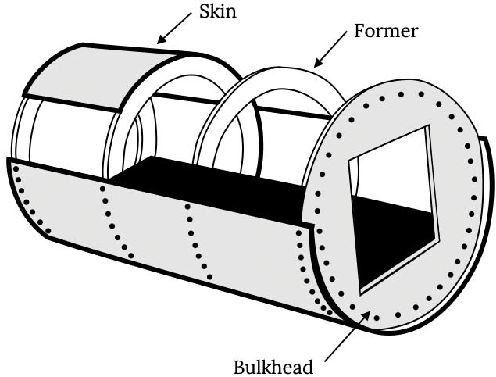
\includegraphics{Figure_1-2.pdf}
}{\caption{Monocoque fuselage structure with transverse stiffeners.\label{fig1.2}}}}

\vspace*{-1\baselineskip}

\section{Monocoque and semimonocoque constructions}

Most flight vehicle structures are thin shells with the cover skin
providing the aerodynamic shape. Monocoque refers to a shell
without supporting stiffening members, whose origin is from the
twentieth-century Greek word ``mono'' meaning alone, plus the
French ``coque'' meaning shell. See figure \ref{fig1.2} The wall of a
monocoque structure has to be strong enough to resist bending and
compressive and torsional loads without buckling. The challenge in
monocoque design is maintaining strength within allowable weight
limits. Another difficulty with monocoque structure is how to
design it to accommodate concentrated loads such as engine
mountings and wing-fuselage interface, which may require the
incorporation of formers (frames) and bulkheads. For large
cross-sectional dimensions the skin of a monocoque structure must
be relatively thick. A more efficient type of construction is one which contains
stiffening members that permit a thinner skin. Also, stiffening
members can be used to diffuse concentrated loads into the skin. A
stiffened thin-walled shell is called semimonocoque. A
semimonocoque body structure and wing structure are shown in
figure \ref{fig1.3}. Both the body structure figure\ref{fig1.3}(a) and the wing
structure in figure \ref{fig1.3}(b) have longitudinal stiffening members
and transverse stiffening members supporting thin skins.



{\def\thefigure{1.3}
\processfigure{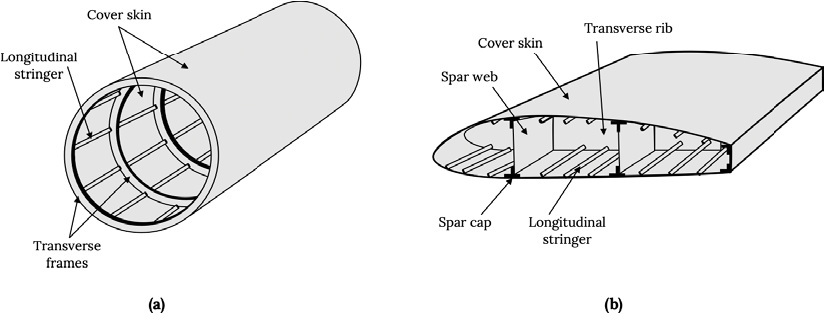
\includegraphics{Figure_1-3.pdf}
}{\caption{(a) Semimonocoque body structure. (b) Semimonocoque wing
structure.\label{fig1.3}}}}


Longitudinal members are called longitudinals, stringers, or stiffeners.
Longerons are longitudinal members having a large cross section.
Longitudinal members act with the skin to resist applied bending and axial
loads. Transverse members in a body structure are known as frames, rings,
and if they cover most of the cross section they are called bulkheads.
Pressure bulkheads cover the entire cross section. Frame members maintain
cross-sectional shape and are used to distribute concentrated loads to the
skin.

In a wing the longitudinal member is called a spar, and it consists of the
spar web and spar cap. The spar cap act with the skin to resists axial and
bending loads applied to the wing. The skin and the spar web develop
shearing stresses to resist torsion and transverse shear due to bending.
Transverse members in a wing are called ribs, and they act to maintain the
airfoil shape. Ribs act with the skin and longitudinals in resisting
circumferential loads due to pressurization.

Longitudinal and transverse members also function to divide the skin into
smaller panels to increase the buckling strength. (See Example \ref{ex11.5} on
page~\pageref{ex11.5}.)




Additional components of a wing are shown in figure \ref{fig1.4}. The internal wing structure consists of spars, ribs, and stringers. The
external wing structure is the skin. Ribs are also used in ailerons,
elevators (flaps), fins, and stabilizers. In a fixed-wing aircraft, the spar
is the main structural member connected to the fuselage at its root and
running spanwise to the tip of the wing. It bends in transmitting the lift
due to flight loads acting on the wing. The flight loads acting on a wing
not only cause bending, but a significant amount of torsion/ twisting of the
wing as well. The skin and shear webs form closed cells in a wing, and
torsion is resisted by shear stresses developed in the wall of these cells.

{\def\thefigure{1.4}
\processfigure{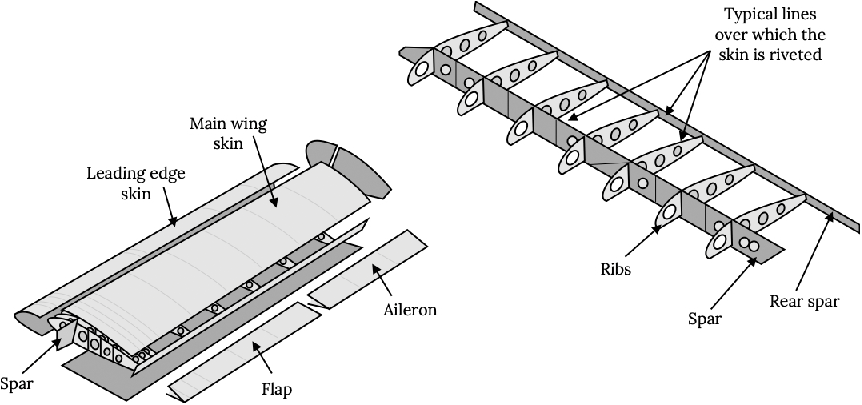
\includegraphics{Figure_1-4.pdf}
}{\caption{Nomenclature for a typical wing structure.\label{fig1.4}}}}

%\clearpage
%\thispagestyle{empty}
%\enlargethispage{1\baselineskip}
{\def\thefigure{1.5}
\processfigure[t]{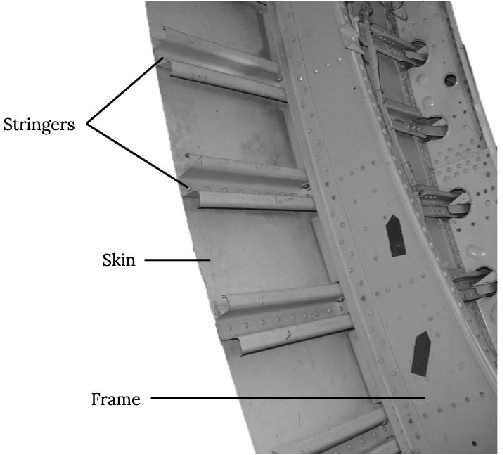
\includegraphics{Figure_1-5.pdf}
}{\caption{Semi monocoque fuselage structure.\label{fig1.5}}}}


%\clearpage

A semimonocoque fuselage structure for a transport aircraft is shown in
figure \ref{fig1.5}. The skin is stiffened by
longitudinal stringers, spaced six to ten inches apart, which function to
increase the buckling strength of the skin and resist fuselage bending
loads. Transverse frames maintain the shape of the fuselage and are
typically spaced twenty inches apart (Young, 2011).

%\vspace*{-\baselineskip}

\section{Rocket structure}

A full-scale rocket consists of a launch vehicle and payload. There are four
major systems in a full-scale rocket: the structural system, the payload
system, the guidance system, and the propulsion system. The structural
system includes the cylindrical body, the fairings, and any control fins.
The payload is the entire spacecraft such\break as a \text{satellite}, experiment, or
whatever else is being lifted into space. When a spacecraft is to be
launched by an expendable booster, a booster adapter, or a launch-vehicle
adapter, structurally links the spacecraft to the launch vehicle. The
payload and its structure is protected by a fairing. Also, refer to the
configuration of the Atlas I launch vehicle shown in figure \ref{fig18.1} on
page~\pageref{fig18.1}. Atlas I consists of an expendable booster and an expendable second
stage.

The cylindrical body of the launch vehicle, or frame, has a thin skin to
reduce weight. Engine thrust is the dominate load that causes compression in
the rocket parts. The buckling resistance of the thin skins is increased
under compression loading by a grid of internal stiffening members attached
to the skins similar to those shown in
figure \ref{fig1.3}(a). The buckling loads for
axially compressed cylindrical shells in experiments are significantly less
than the buckling load determined from an analysis of the perfect structure.
Imperfection in the shell geometry is main the reason for the discrepancy
between theory and experiment Refer to the discussion at the end of article
\ref{sec10.2.1} on page~\pageref{sec10.2.1}. The buckling knockdown factor (KDF) has been introduced
to reduce the buckling load predicted by the analysis of the prefect
structure to aid in the structural design (Hilburger, 2018).

{\def\thefigure{1.6}
\processfigure[H]{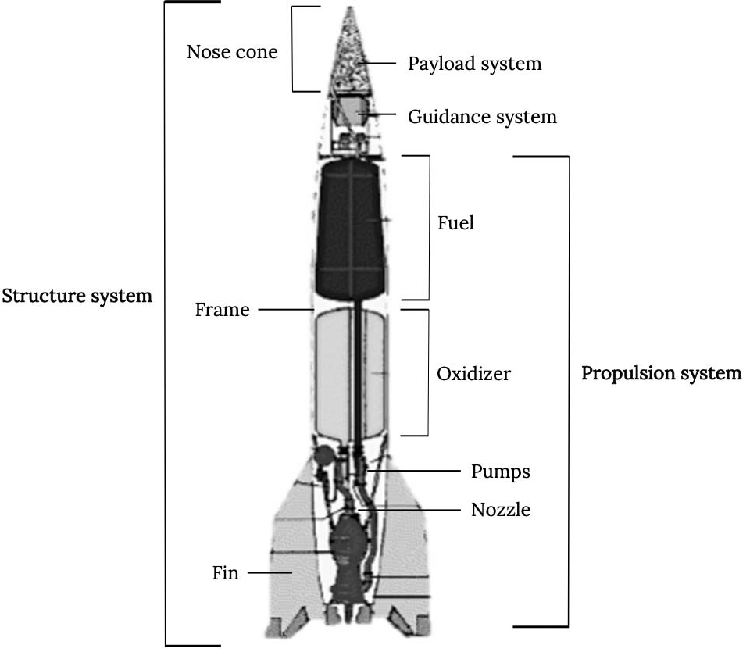
\includegraphics{Figure_1-6.pdf}
}{\caption{Rocket systems and components.\label{fig1.6}}}}


\begin{thebibliography}{}
\bibitem{}
Ashby, M. F., \textbf{\textit{Materials Selection in Mechanical Design}}.
Oxford: Pergamon Press, 1992.

\bibitem{}
Curtis, Howard D., \textbf{\textit{Fundamentals of Aircraft Structural
Analysis}}. Jefferson City, MO: Richard D. Irwin, a Times Mirror Higher
Education Group, Inc. Company, 1997, pp. 1--34.

\bibitem{}
Hilburger, M. W., ``\textbf{\textit{On the Development of Shell Buckling
Knockdown Factors for Stiffened Metallic Launch Vehicle Cylinders}}.''
Presented at the 2018 AIAA/ASCE/AHS/ASC Structures, Structural Dynamics, and
Materials Conference, Kissimmee FL, AIAA 2018-1990. Washington, DC: American
Institute of Aeronautics and Astronautics, 2018.

\bibitem{}
Young, Richard, ``\textbf{\textit{Fuselage Design 101: Basic Terms and
Concepts}}.'' Presented at the NTSB Airplane Structural Integrity Forum,
Washington, D. C., September 21, 2011.
\end{thebibliography}

\clearemptydoublepage

\end{document}